\section{Experiments}
\label{sec:experiments}

\subsection{Setup}
\label{sec:setup}

\paragraph{Model and training.} We train MAML with the Conv4 backbone (four $3{\times}3$ conv + BatchNorm + ReLU + $2{\times}2$ maxpool blocks) under \citeauthor{finn2017model}'s original protocol \citep{finn2017model}: inner-loop rate $\alpha{=}0.01$, Adam outer-loop rate $\beta{=}0.001$, $T_{\text{train}}{=}5$ / $T_{\text{test}}{=}10$ steps, meta-batch size 4, 60{,}000 iterations, 5-way 1-shot; all results use the converged checkpoint at $T{=}T_{\text{test}}$. For \biadt and both sanity checks (\Cref{tab:biadt,tab:sanity}) we additionally train a ResNet-10 backbone \citep{he2016deep} (4 residual blocks) under the identical protocol, to test whether Conv4's margins are a resolution artifact.

\paragraph{Datasets.} \emph{miniImageNet} \citep{ravi2017optimization}: 100 ImageNet classes, 600 images each, 64/16/20 split. \emph{tieredImageNet} \citep{ren2018meta}: a larger, WordNet-hierarchy-split variant (608 classes) whose semantically distant test classes make it our primary benchmark. \emph{CUB-200-2011} \citep{welinder2010caltech}: 200 fine-grained bird species, a stress test for negative transfer and our OOD probe.

\paragraph{Protocol.} All three quantitative checks (\Cref{sec:biadt,sec:sanity}) run on $N{=}600$ sampled tieredImageNet meta-test tasks, $\Delta M$ estimated per task via stratified bootstrap query sets; CUB-200-2011 supplies the OOD condition for the support-set sanity check. We report mean $\pm$ MoE, the half-width of a 96\% bootstrap percentile CI (10{,}000 resamples), and test \biadt significance with a one-sided one-sample $t$-test against zero. For qualitative analysis we run \fama on 600 further cross-domain tasks each for mini2cub and tiered2cub.

\subsection{Quantitative Results}
\label{sec:quant_results}

\begin{table}[t]
\centering\footnotesize
\caption{\biadt on tieredImageNet ($N{=}600$ tasks per backbone, identical protocol): both directions are positive and significant for both backbones (one-sided one-sample $t$-test against 0), confirming $\Phi_{\mathrm{FAMA}}$'s sign is causally linked to $\Delta M$ regardless of architecture.}
\label{tab:biadt}
\renewcommand{\arraystretch}{0.8}
\begin{tabular}{@{}lcc@{}}
\toprule
Metric & Mean $\pm$ MoE & $p$-value \\
\midrule
\multicolumn{3}{@{}l}{\textit{(a) Conv4}} \\
$\mathrm{ABC}_\downarrow$ & $0.186 \pm 0.109$ & $1.99{\times}10^{-4}$ \\
$\mathrm{ABC}_\uparrow$   & $0.289 \pm 0.122$ & $7.01{\times}10^{-7}$ \\
\multicolumn{3}{@{}l}{\textit{(b) ResNet-10}} \\
$\mathrm{ABC}_\downarrow$ & $0.374 \pm 0.105$ & $2.07{\times}10^{-13}$ \\
$\mathrm{ABC}_\uparrow$   & $0.695 \pm 0.120$ & $1.10{\times}10^{-29}$ \\
\bottomrule
\end{tabular}
\end{table}

\paragraph{\biadt (\Cref{tab:biadt}).} Both directions are positive with $p<0.001$ for both backbones: deleting superpixels in either direction indicated by $\Phi_{\mathrm{FAMA}}$ shifts $\Delta M$ significantly faster than random deletion, and $\mathrm{ABC}_\uparrow$'s cleaner separation suggests the harmful-region signal is easier to localize. Conv4's margins are wide ($\sim$59\% of the mean for $\mathrm{ABC}_\downarrow$, \Cref{tab:biadt}a), consistent with its coarse feature grid: bilinear upsampling (\Cref{eq:branch_saliency}) blurs boundaries and adds variance without flipping the effect's sign (\Cref{sec:limitations}). ResNet-10 (\Cref{tab:biadt}b) is a direct test of that explanation: same protocol, same tasks, only the backbone changes, and both margins tighten while both effects strengthen by several orders of magnitude in $p$-value -- exactly what a resolution artifact predicts, not what a faithfulness failure would show.

\begin{table}[t]
\centering\footnotesize
\caption{Sanity checks on tieredImageNet ($N{=}600$; Spearman~/~Pearson correlation against the unperturbed $\Phi_{\mathrm{FAMA}}$, mean $\pm$ MoE, both backbones). \textbf{Top:} cascading randomization of $\theta_0^b$ collapses to the noise floor as soon as the output-nearest block is destroyed. \textbf{Bottom:} all three $S_i$ interventions shift the map significantly below the near-1 correlation of a content-blind detector.}
\label{tab:sanity}
\renewcommand{\arraystretch}{0.72}
\begin{tabular}{@{}lcccc@{}}
\toprule
& \multicolumn{2}{c}{Conv4} & \multicolumn{2}{c}{ResNet-10} \\
\cmidrule(lr){2-3}\cmidrule(lr){4-5}
\multicolumn{5}{@{}l}{\textit{(a) Cascading randomization of $\theta_0^{b}$}} \\
Destroyed block & Spearman & Pearson & Spearman & Pearson \\
\midrule
none (head only) & $0.085\pm.016$ & $0.087\pm.016$ & $0.081\pm.017$ & $0.084\pm.018$ \\
block 4 & $-0.010\pm.012$ & $-0.012\pm.012$ & $-0.000\pm.011$ & $0.000\pm.011$ \\
block 3 & $-0.008\pm.012$ & $-0.007\pm.013$ & $-0.008\pm.011$ & $-0.005\pm.011$ \\
block 2 & $-0.013\pm.012$ & $-0.013\pm.012$ & $-0.001\pm.011$ & $-0.002\pm.011$ \\
block 1 & $-0.006\pm.012$ & $-0.005\pm.012$ & $-0.009\pm.011$ & $-0.010\pm.011$ \\
\midrule
\multicolumn{5}{@{}l}{\textit{(b) Intervention on $S_i$}} \\
Scenario & Spearman & Pearson & Spearman & Pearson \\
\midrule
OOD task mixing    & $0.330\pm.018$ & $0.340\pm.018$ & $0.289\pm.017$ & $0.296\pm.018$ \\
Label permutation  & $0.250\pm.023$ & $0.258\pm.024$ & $0.191\pm.020$ & $0.195\pm.021$ \\
Hard task (blur)   & $0.258\pm.016$ & $0.266\pm.016$ & $0.232\pm.015$ & $0.241\pm.016$ \\
\bottomrule
\end{tabular}
\end{table}

\paragraph{Randomizing $\theta_0$ (\Cref{tab:sanity}a).} Correlation collapses from $\approx\!0.09$ to $\approx\!0$ the instant the output-nearest block is randomized, then stays flat, on both backbones. This could look like a resolution artifact, so we isolated it with a control: replacing $\Delta M$ with $\Delta M':=\mathbb{E}_{Q_i}[\mathcal{L}(Q_i,\theta_0)-\mathcal{L}(Q_i,\phi_T)]$ (\emph{any} adaptation vs.\ none) reproduces the same sweep as a \emph{smooth}, monotonic decay from $0.650$ (head) to $0.075$ (deepest block) -- a linear head still exploits generic texture structure even a random conv stack produces. Per \citet{adebayo2018sanity}, a gently-decaying map is the \emph{failure} signature; \fama's two-branch subtraction (\Cref{eq:fama_final}) cancels that floor, as \Cref{prop:decomposition} predicts.

\paragraph{Intervening on $S_i$ (\Cref{tab:sanity}b).} All three interventions pull correlation well below a content-blind map, on both backbones, in the same order: OOD mixing disrupts least, label permutation most -- permutation and blur corrupt the \emph{supervisory signal} used at every $T$ adjoint step, compounding across the trajectory, whereas OOD mixing keeps each image-label pair internally consistent, so each step stays locally "valid," and both backbones are shallow enough that CUB and tieredImageNet, though disjoint, share low-level texture statistics.

\subsection{Qualitative Case Studies}
\label{sec:qual_results}

\begin{figure}[t]
    \centering
    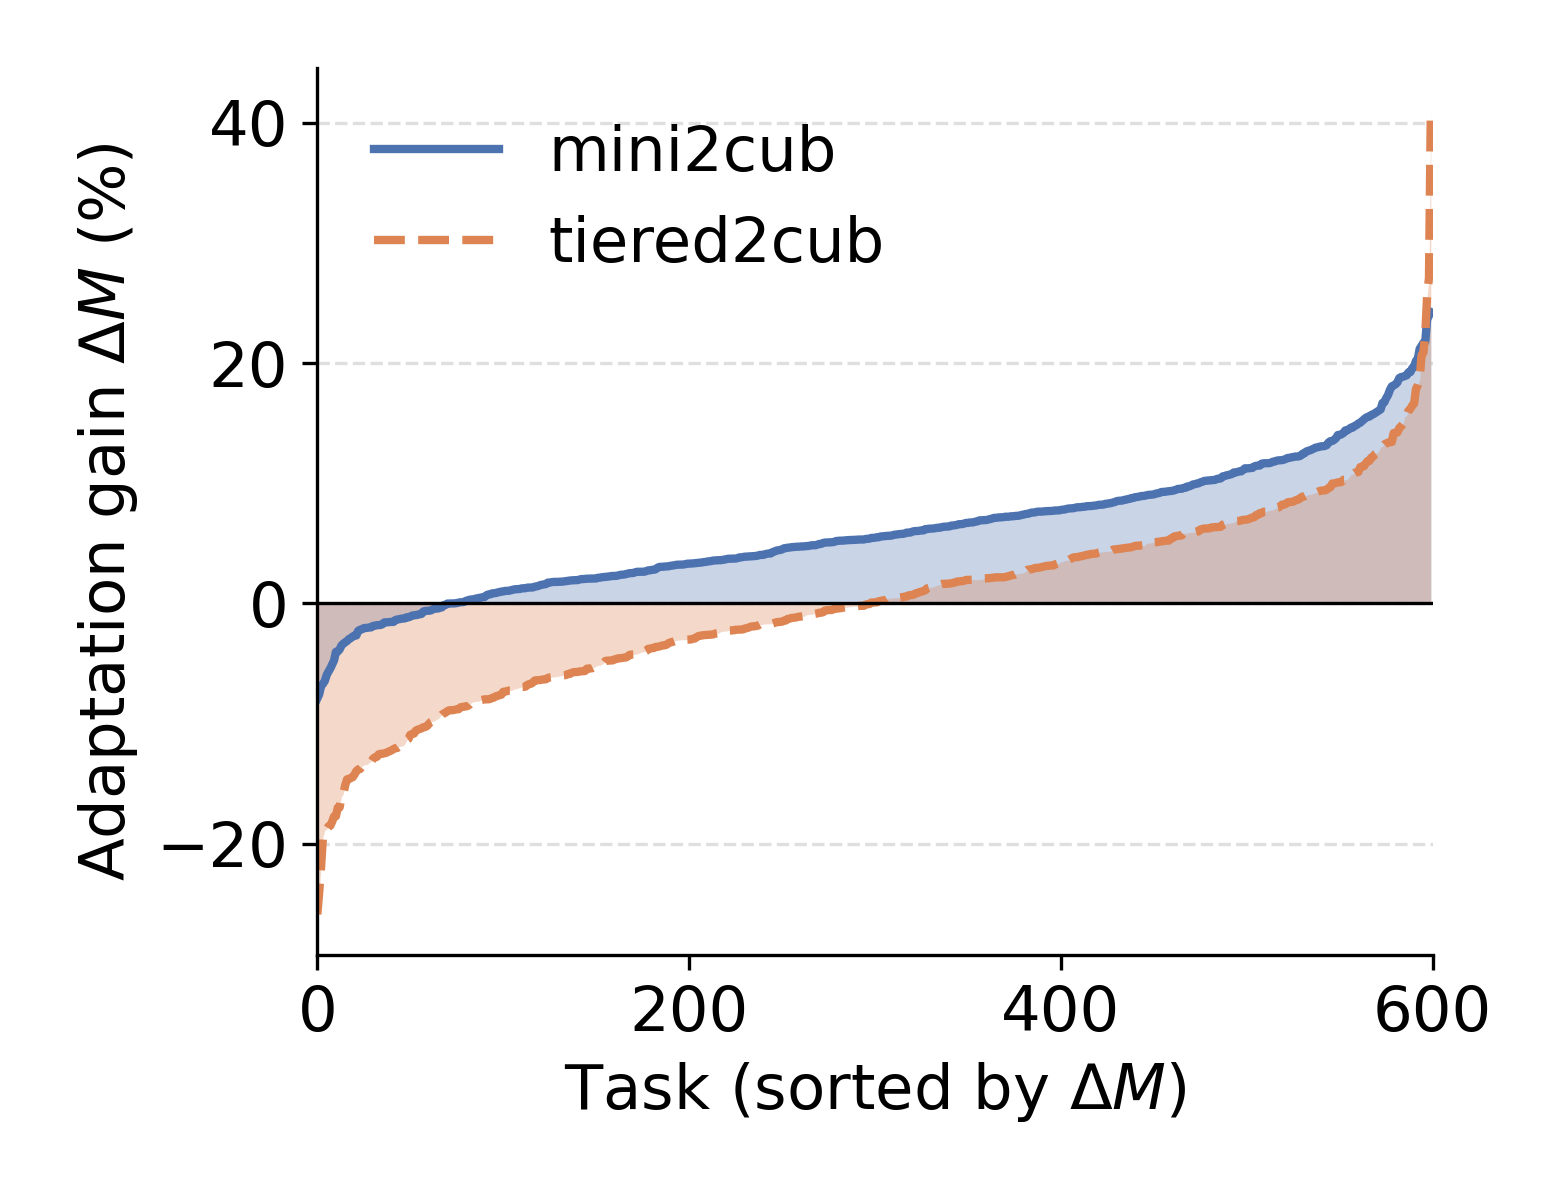
\includegraphics[width=0.4\linewidth]{figures/delta_m_distribution.png}
    \caption{Sorted $\Delta M$ over 600 tasks per benchmark. tiered2cub is both wider (tails at $-25.88\%$/$+41.24\%$ vs.\ $-7.91\%$/$+24.24\%$) and far more often negative (49.7\% of tasks vs.\ 12.5\%), consistent with tieredImageNet's category-level split yielding broader but less fine-grained prior knowledge.}
    \label{fig:delta_m_dist}
\end{figure}

\Cref{fig:delta_m_dist} sorts $\Delta M$ over 600 sampled tasks for both cross-domain settings. tiered2cub is both wider and far more negative-heavy than mini2cub, matching tieredImageNet's coarser, category-level prior: it generalizes broadly but lacks fine-grained specialization for CUB's subtle inter-species boundaries, so backbone adaptation becomes higher-variance.

\begin{figure}[t]
    \centering
    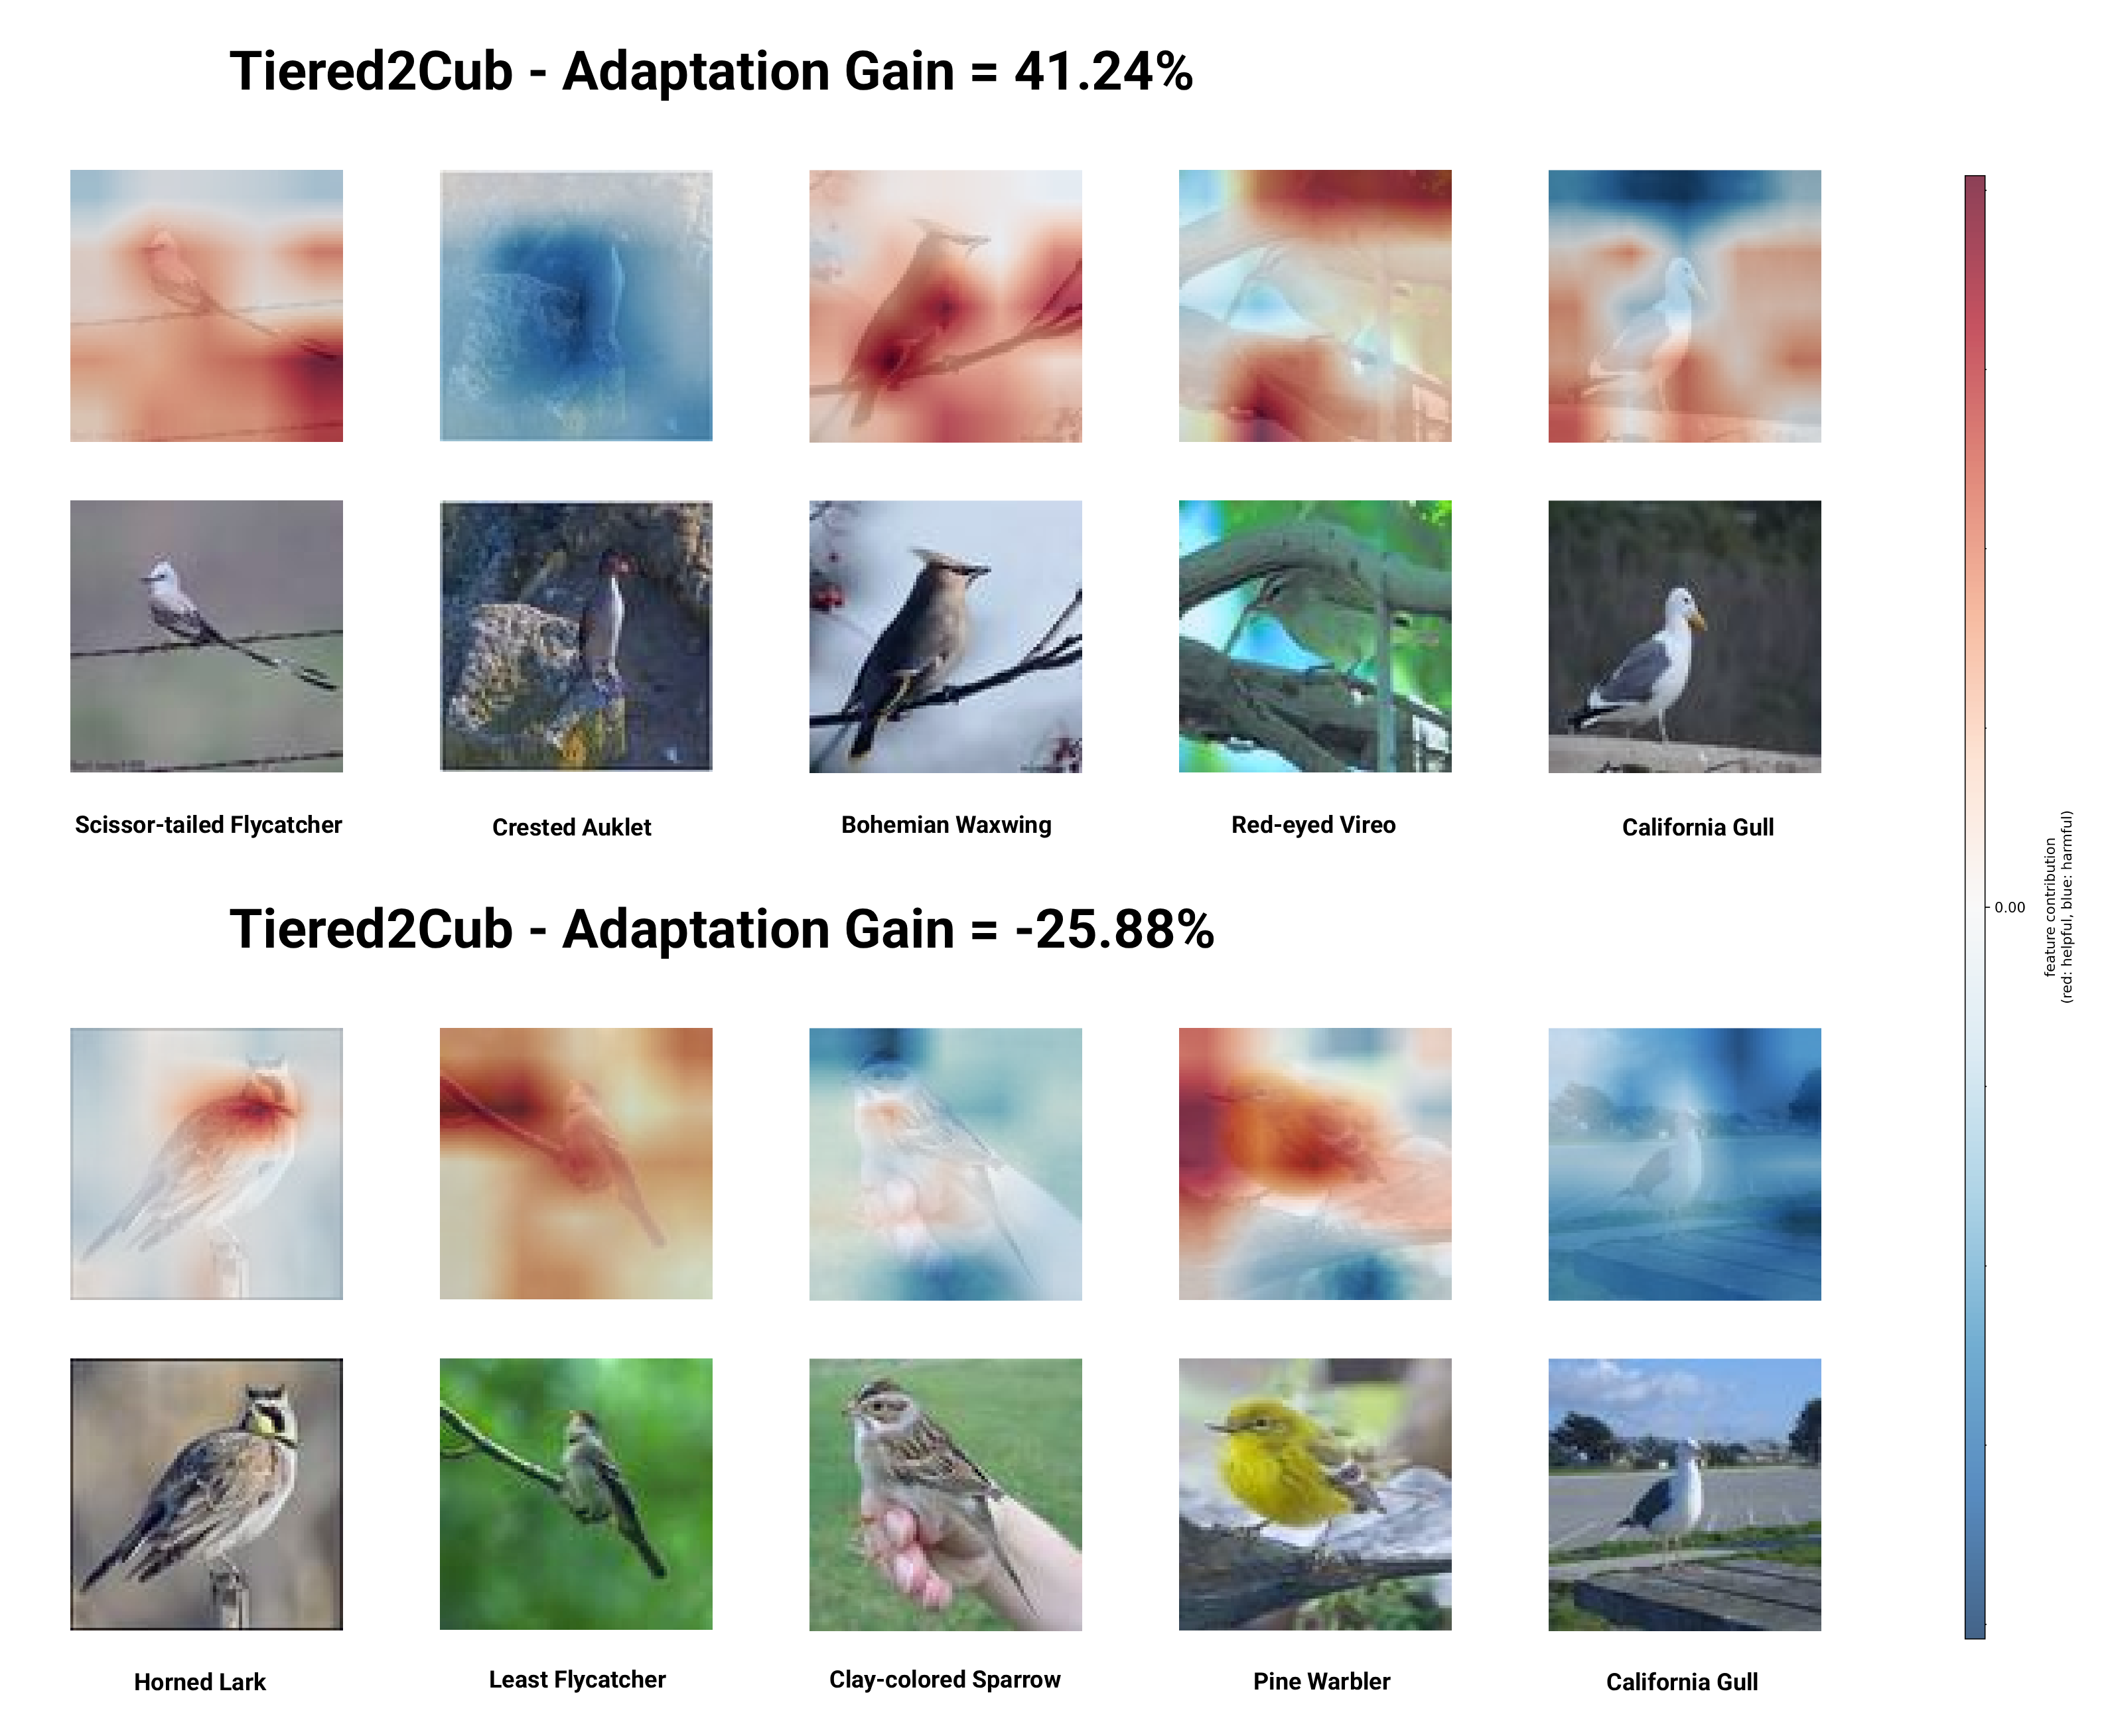
\includegraphics[width=0.32\linewidth]{figures/tiered2cub_lmag.png}
    \caption{$\Phi_{\mathrm{FAMA}}$ on the most positive- (top) and most negative-transfer (bottom) tiered2cub tasks (red: helpful, blue: harmful). Positive cases lock onto discriminative body/plumage regions; negative cases spend their attribution budget on background, occlusion, or artifacts instead of the bird.}
    \label{fig:case_study}
\end{figure}

\Cref{fig:case_study} shows the extreme tasks from \Cref{fig:delta_m_dist} (mini2cub counterparts in \Cref{app:qual}); three patterns recur across both tails. \textbf{(1) Contextual bias.} On plain backgrounds, positive-transfer maps lock onto the bird (\emph{Bohemian Waxwing}) or a discriminative part (\emph{Horned Lark}'s plumes); when the subject is indistinct or occluded, red shifts onto branches or foliage (\emph{Scissor-tailed Flycatcher}, \emph{Crested Auklet}) -- the backbone falls back on background correlations exactly when the object is a weak signal. \textbf{(2) Artifact sensitivity.} Blue attribution lands on non-biological confounds: color noise, clutter, or a hand holding the bird -- evidence $\Phi_{\mathrm{FAMA}}$ tracks image content, not a class template (\emph{California Gull} appears in both extremes with near-opposite structure). \textbf{(3) Spatial bleeding.} For small subjects, attribution leaks past the object boundary -- the qualitative counterpart of \Cref{tab:biadt}'s wide margins, and likewise a resolution artifact rather than a sign error.

Contextual bias here is a case-study observation, not a population-level statistic: \Cref{fig:case_study} covers only the selected extreme tasks. A direct quantitative test needs no new machinery -- CUB-200-2011 ships a bounding box per image, so the \emph{object sign-agreement rate} (the fraction of $\Phi_{\mathrm{FAMA}}$'s positive mass inside versus outside it, correlated against $\Delta M$ over all 600 tasks) would make this population-level.
